

%%%%%%%%%%%%%%%%%%%%%%%%%%%%%%%%%%%%%%%%%
% University/School Laboratory Report
% LaTeX Template
% Version 3.1 (25/3/14)
%
% This template has been downloaded from:
% http://www.LaTeXTemplates.com
%
% Original author:
% Linux and Unix Users Group at Virginia Tech Wiki 
% (https://vtluug.org/wiki/Example_LaTeX_chem_lab_report)
%
% License:
% CC BY-NC-SA 3.0 (http://creativecommons.org/licenses/by-nc-sa/3.0/)
%
%%%%%%%%%%%%%%%%%%%%%%%%%%%%%%%%%%%%%%%%%

%----------------------------------------------------------------------------------------
%	PACKAGES AND DOCUMENT CONFIGURATIONS
%----------------------------------------------------------------------------------------

\documentclass{article}

\usepackage[version=3]{mhchem} % Package for chemical equation typesetting
\usepackage{siunitx} % Provides the \SI{}{} and \si{} command for typesetting SI units
\usepackage{graphicx} % Required for the inclusion of images
\usepackage{natbib} % Required to change bibliography style to APA
\usepackage{amsmath} % Required for some math elements 
\usepackage{listings}
\usepackage{color}
\usepackage{caption}
\usepackage{rotating}


\definecolor{dkgreen}{rgb}{0,0.6,0}
\definecolor{gray}{rgb}{0.5,0.5,0.5}
\definecolor{mauve}{rgb}{0.58,0,0.82}

\lstset{frame=tb,
  language=Java,
  aboveskip=3mm,
  belowskip=3mm,
  showstringspaces=false,
  columns=flexible,
  basicstyle={\small\ttfamily},
  numbers=none,
  numberstyle=\tiny\color{gray},
  keywordstyle=\color{blue},
  commentstyle=\color{dkgreen},
  stringstyle=\color{mauve},
  breaklines=true,
  breakatwhitespace=true,
  tabsize=3
}
\setlength\parindent{0pt} % Removes all indentation from paragraphs

\renewcommand{\labelenumi}{\alph{enumi}.} % Make numbering in the enumerate environment by letter rather than number (e.g. section 6)

%\usepackage{times} % Uncomment to use the Times New Roman font

%----------------------------------------------------s------------------------------------
%	DOCUMENT INFORMATION
%----------------------------------------------------------------------------------------

\title{Laboratory Assignment 3 Write Up \\ Computer Science 441} % Title

\author{\textsc{Andreas Bach Landgrebe} \\
\textsc{Francis Craft} \\
\textsc{Troy Dinga}} % Author name

\date{\today} % Date for the report

\begin{document}

\maketitle % Insert the title, author and date

\begin{center}
\begin{tabular}{l r}
Date Submitted:  February 22, 2016 \\ % Date the experiment was performed
Partners:  Andreas Bach Landgrebe \& Francis Craft \\ \& Troy Dinga \\ % Partner names
Instructor:  Dr. Gregory M. Kapfhammer  % Instructor/supervisor
\end{tabular}
\end{center}

% If you wish to include an abstract, uncomment the lines below
% \begin{abstract}
% Abstract text
% \end{abstract}

%----------------------------------------------------------------------------------------
%	SECTION 1
%----------------------------------------------------------------------------------------

\section{A detailed listing of the commands that you typed to perform compression and file transfer.}

The first commands that were used in this lab were those used to compress the Java archives. The Zip, Pack200, and Pack200 + Gzip tools required the use of the following basic terminal commands within the working directory containing the archives in question: 

\begin{itemize}
	\item Zip: \texttt{zip nameOfZippedFileNoExtension archive.jar}
	\item Pack200: \texttt{pack200 --no-gzip nameOfPackedFile.pack archive.jar}
	\item Pack200 + Gzip: \texttt{pack200 nameOfPackedFile.pack.gz archive.jar}
\end{itemize}

In order to time these compressions, the \texttt{time} command was added before each of the above lines when actually running their commands. 

\vspace{3mm}

In order to transfer files, we first set up an HTTP server using the command 
\texttt{python -m SimpleHTTPServer 4200}. After this, we were able to download whichever files we wanted from the server using \texttt{wget 0.0.0.0:4200/filename.jar} in a separate terminal window. 

%----------------------------------------------------------------------------------------
%	SECTION 2
%----------------------------------------------------------------------------------------

\section{Using both text and diagrams, a description of client-server communication with compression.}

The below diagram illustrates the communication of a client-server interaction with compression.

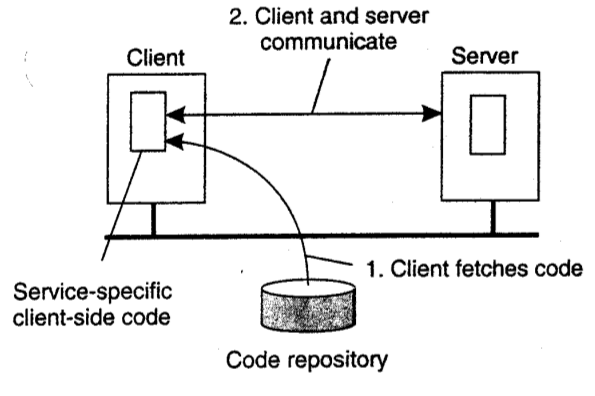
\includegraphics[scale=0.5]{figure317.png}

There can a couple of different approaches to perform comporession from a client-server communication. One approach is to have the client-side implementation use a proprietary protocol \cite{tanenbaum_steen_2007}. However, this requires that software would have to be available to the client at the time the client application is being developed \cite{tanenbaum_steen_2007}. An alternative to this approach is allowed the server provide the implementation of the client when the client binds to the server. This step of the process can also be seen as the request process between the client and the server when the client is requesting a process to occur from the server. When this point occurs, the client will download the implementation and invoke the server \cite{tanenbaum_steen_2007}. The whole principle is what is shown in the above diagram between the client and the sever. In the diagram, the first step that occurs is that the client fetches the code. Before that could even happen, however, the server needs to start up. The command of ``python -m SimpleHTTPServer 4200" allows the server to be able to start up to accept HTTP protoocol the transfer files. After the server is started up and waits for request and the client fetches code from a version control repository, the client and server communicate. This is done from the laboratory assignment from using the wget program. The whole idea behind this dynamic approach is to have the client first fetcher the software and then the client will invoke the server \cite{tanenbaum_steen_2007}.

%----------------------------------------------------------------------------------------
%	SECTION 3
%----------------------------------------------------------------------------------------
\section{A full-featured description of all of the equations for this assignment’s evaluation metrics.}

The time taken by each of the compression techniques to actually perform the compression on each of ten different \texttt{.jar} files was recorded by using the \texttt{time} command. We ran five of these compressions in each instance and found both the mean and standard deviation of each of these sets of trials. The mean was found by finding the sum of the elapsed time values and dividing them by the number of iterations - in this case, five. The standard deviation involved the finding the mean of the differences between the mean of the trial times and each individual time. 

\vspace{3mm}

The percentage change in the size of the files after compression as compared to their original size was also recorded. This was done by dividing the difference between the two sizes by the original size and multiplying the resulting decimal by 100.

%----------------------------------------------------------------------------------------
%	SECTION 4
%----------------------------------------------------------------------------------------

\section{A detailed paper that reports on the empirical results arising from the use of the benchmarks.}

The data from this lab is compiled in Section 7 of this report. This data was gathered using the following ten JAR files:
JavaRunner.jar,  p6spy.jar, ccl.jar, jcommander-1.33-SNAPSHOT.jar, hsqldb.jar, jdepend-2.9.1.jar, jacocoant.jar, jhbasic.jar, javacc.jar, javancss.jar.


\par
The information gathered during this lab points, using two different types of data, to the fact the Zip does not compress a JAR file as extensively as Pack200 or Pack200+GZip. This fact became visible firstly in the times it takes for Zip to compress. In the times it took Zip to compress the ten JAR files never have a mean value exceeding the time it took Pack200 or Pack200+GZip. This is complimented by the fact that the percent reduction of Zip is often far exceeded by Pack200+GZip. The lack of compression compared to Pack200+GZip led Troy and Francis to question Andreas when the percent reduction was being calculated. After determining the Zip percent reductions, Troy and Francis did not believe the validaty of Pack200+GZip's compression percentage until they saw the math. To them, the reduction rates of Pack200+GZip seemed incorrectly calculated they were so much larger.

%----------------------------------------------------------------------------------------
%	SECTION 5
%----------------------------------------------------------------------------------------
\section{A description of the challenges that you encountered when completing this assignment.}

The challenges we faced while completing this lab are those related to our part- nership. Unlike other groups, ours was a group of 3, and two members of the group are not in lab at the same time. This added an extra level of difficulty to communication. Though this challenge was easily over come. The next chal- lenge came from the fact that with the three of us working at times all at once, there were two different merge conflicts. These tripped up the group for short periods of time. Thankfully the group was comprised of two seniors and one junior who have had plenty of experience working in groups, over coming merge conflicts, and testing the effectiveness of the different compression algorithms.


%----------------------------------------------------------------------------------------
%	SECTION 6
%----------------------------------------------------------------------------------------
\section{A detailed listing of the tasks completed by each of the member of your partnership.}

Each group member was able to complete each of the tasks in an ordered fashion. When running the experiments the test the effectiveness of the different compression algorithms, Troy Dinga was responsible for conducting experiements for the zip compression algorithm. Francis Craft was responsible for running the Pack200 compression algorithm. Andreas Landgrebe was responsible for running the Pack200+Gzip compression algothim. After this occurred, each group member was responsible for calculating the percentage change in the different compression algorithms on how much smaller these files had become. Andreas was responsible for calculating the changes for the Pack200+Gzip files. Francis and Troy were working together in calculating the percentages on the zip compression algorithm. Andreas Landgrebe was responsible for adding all of the jar files to the repository. Francis and Troy were responsible in figuring out how to work with the localhost web server and learn the commands on how to use wget. 

%----------------------------------------------------------------------------------------
%	SECTION 7
%----------------------------------------------------------------------------------------
\section{Tables}


\begin{figure}
\caption{Zip Compression Time, in seconds}
\begin{sideways}
\begin{tabular}{l l l l l l l l l l l }
	  & JavaRunner & p6spy & ccl & hsqldb & jacocoant & javacc & javancss & jcommander & jdepend & jhbasic \\ \hline
1&	0.017 &	0.056 & 0.1 &	0.254 &	0.115 &	0.076 &	0.085 &	0.029 &	0.03&	0.063 \\
2&  0.017 &	0.043 &	0.086&	0.418 &	0.104 &	0.076 &	0.086 &	0.031 &	0.029&	0.065 \\
3&	0.016 &	0.04  &	0.09 &  0.238 &	0.107 &	0.075 &	0.084 &	0.028 &	0.029&	0.065 \\
4&	0.016 &	0.042 &	0.086&	0.228 &	0.103 &	0.075 &	0.086 &	0.03  &	0.031&	0.064 \\
5&	0.016 &	0.049 &	0.086&	0.233 &	0.101 &	0.079 &	0.084 &	0.033 &	0.029&	0.063 \\
Mean&0.0164&	0.046 &	0.0896&	0.2742&	0.106 &	0.0762&	0.085 &	0.0302&	0.0296&	0.064 \\
Standard Dev.&	1.58&	0.00&	0.01&	0.01&	0.08&	0.01&	0.0	&0.00&	0.00&	0.00 
\end{tabular}
\end{sideways}
\end{figure}

\begin{figure}
\caption{Pack200 Compression Time, in seconds}
\begin{sideways}
\begin{tabular}{l l l l l l l l l l l }
	  & JavaRunner & p6spy & ccl & hsqldb & jacocoant & javacc & javancss & jcommander & jdepend & jhbasic \\ \hline
1 &	0.25	&1.08&	2.2&	3.354&	1.164&	1.45&	1.277&	0.62&	0.492&	1.238 \\
2&	0.25&	0.91&	2.13&	3.431&	1.169&	1.091&	1.141&	0.72&	0.428&	0.945\\
3&	0.26&	1.17&	2.18&	3.51&	1.062&	1.203&	1.327&	0.67&	0.481&	0.818\\
4&	0.22&	1.02&	2.37&	3.404&	1.041&	1.141&	1.252&	0.67&	0.432&	0.925\\
5&	0.23&	1.05&	2.21&	3.423&	1.037&	1.11&	1.334&	0.64&	0.483&	0.848\\
Mean&	0.242&	1.046&	2.218&	3.4244&	1.0946&	1.199&	1.2662&	0.664&	0.4632&	0.9548\\
Standard Dev.&	1.58&	0.02&	0.09&	0.09&	0.06&	0.07&	0.15&	0.08&	0.04&	0.03 
\end{tabular}
\end{sideways}
\end{figure}

\begin{figure}
\caption{Pack200+GZip Compression Time, in seconds}
\begin{sideways}
\begin{tabular}{l l l l l l l l l l l }
	  & JavaRunner & p6spy & ccl & hsqldb & jacocoant & javacc & javancss & jcommander & jdepend & jhbasic \\ \hline
1	&0.3	&1.2&	2.33&	6.56	&1.83	&1.81	&2.38&	0.67	&0.74	&1.57\\
2	&0.24&	0.88&	2.47&	6.16&	1.6&	1.96&	2.06&	0.73&	0.76	&1.46\\
3	&0.27&	1.14&	2.42	&6.59&	1.77&	1.83	&2.28	&0.73	&0.9	&1.5\\
4	&0.23	&1.19&	2.42	&6.15&	1.6&	2	&2.43	&0.71&	0.86&	1.6\\
5	&0.26	&1.17&	2.26	&6.13&	1.77&	1.97&	2.42	&0.84	&0.88&	1.56\\
Mean&	0.26&	1.116&	2.38	&6.318	&1.714	&1.914&	2.314&	0.736&	0.828&	1.538\\
Standard Dev.&	1.58&0.03&	0.13&	0.08&	0.24&	0.11&	0.09&	0.15	&0.06&	0.07
\end{tabular}
\end{sideways}
\end{figure}

\begin{figure}
\caption{Zip and Pack200+GZip Percent Reductions}
\begin{sideways}
\begin{tabular}{l l l l l l l l l l }
Zip\\ \hline
	  JavaRunner & p6spy & ccl & hsqldb & jacocoant & javacc & javancss & jcommander & jdepend & jhbasic \\ \hline
53.86 &	9.14	&6.32&	5.32&	9.04&	7.52&	2.89&	11.82&	6.67&	8.53\\ \hline
\\
Pack200+GZip \\ \hline
JavaRunner & p6spy & ccl & hsqldb & jacocoant & javacc & javancss & jcommander & jdepend & jhbasic \\ \hline
74.82&	69.57&	66.27&	64.54&	49.12&	60.22&	72.81&	66.83&	67.05&	65.25
\end{tabular}
\end{sideways}
\end{figure}

%----------------------------------------------------------------------------------------
%	BIBLIOGRAPHY
%----------------------------------------------------------------------------------------

\nocite{tanenbaum_steen_2007}

\bibliographystyle{plain}

\bibliography{sample}

%----------------------------------------------------------------------------------------


\end{document}
